\documentclass[journal]{IEEEtran}
\usepackage[spanish,english]{babel}

\usepackage{amssymb, amsmath} %Paquetes matemáticos de la American Mathematical 
\usepackage[utf8]{inputenc}
\usepackage{graphicx}
\usepackage{float}
\usepackage{hyperref}
\usepackage{listings}
\usepackage{xcolor}

\definecolor{codegreen}{rgb}{0,0.6,0}
\definecolor{codegray}{rgb}{0.5,0.5,0.5}
\definecolor{codepurple}{rgb}{0.58,0,0.82}
\definecolor{backcolour}{rgb}{0.95,0.95,0.92}
% Definicio de estilo para el codigo fuente que se cita
\lstdefinestyle{mystyle}{
    backgroundcolor=\color{backcolour},   
    commentstyle=\color{codegreen},
    keywordstyle=\color{magenta},
    numberstyle=\tiny\color{codegray},
    stringstyle=\color{codepurple},
    basicstyle=\ttfamily\footnotesize,
    breakatwhitespace=false,         
    breaklines=true,                 
    captionpos=b,                    
    keepspaces=true,
    numbers=left,                    
    numbersep=5pt,                  
    showspaces=false,                
    showstringspaces=false,
    showtabs=false,                  
    tabsize=2,
}
\lstset{style=mystyle}

\renewcommand{\lstlistingname}{Código}

\ifCLASSINFOpdf

\else

\fi

\hyphenation{op-tical net-works semi-conduc-tor}


\begin{document}

\title{Ejercicio 3 - tema 2 \\ Creación de una base de datos con la instrucción create database}
%
\author{Vicente Romero Andrade}

\markboth{Ejercicio 3 - tema 2 Creación de una base de datos con la instrucción create database, Marzo~2021}%
{Shell \MakeLowercase{\textit{et al.}}: }
% The only time the second header will appear is for the odd numbered pages

\maketitle


\IEEEpeerreviewmaketitle

\section{Objetivo}
% The very first letter is a 2 line initial drop letter followed

\IEEEPARstart{E}{l} objetivo es crear una base de datos a partir de la instrucción create database así como la creación de su diccionario de datos posterior proceso de
configuración realizado en ejercicios anteriores.


\section{Desarrollo}
\subsection{C1. Codigo del script s-03-crea-directorios.sh}
\lstinputlisting[language=sql,caption=s-03-crea-directorios.sh,label={lst:scriptloop}]{s-03-crea-directorios.sh}
\subsection{C2. Codigo del script s-04-crea-bd.sql}
\lstinputlisting[language=sql,caption=s-04-crea-bd.sql,label={lst:scriptpwd}]{s-04-crea-bd.sql}
\subsection{C3. Codigo del script s-05-crea-diccionario-datos.sql}
\lstinputlisting[language=sql,caption=s-05-crea-diccionario-datos.sql,label={lst:scriptpwd}]{s-05-crea-diccionario-datos.sql}
\subsection{C4.  Salida del validador}
\begin{figure}[H]
  \centering
  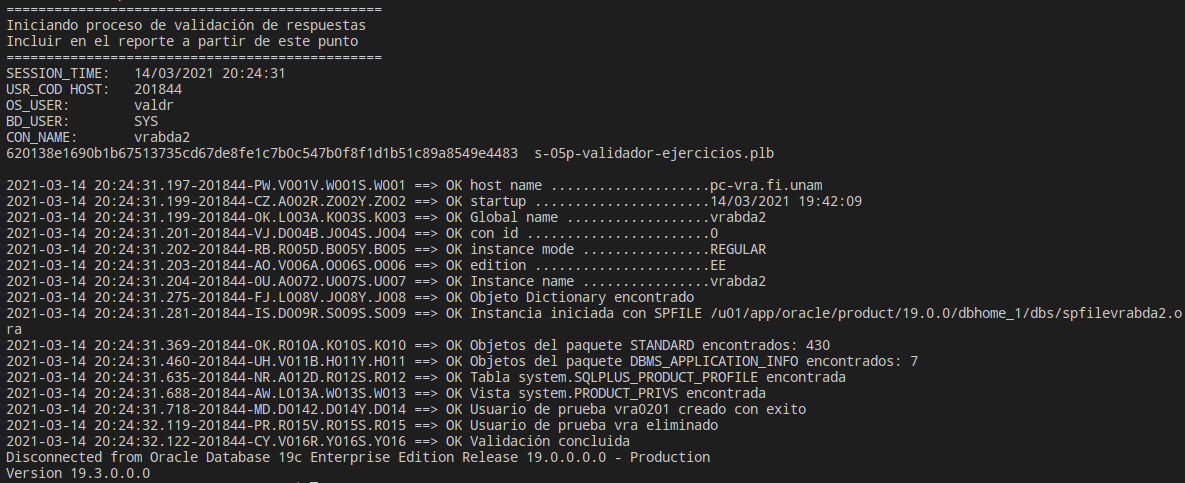
\includegraphics[scale=.21]{validador_ej3_t2.png}
   \caption{Salida del validador}
   \label{fig:salidascript}
\end{figure}
\section{Conclusiones}
En este ejercicio se crearon los directorios donde residirán físicamente los datos de la base,
así como el script que se ejecutara en sql para crear la base de datos usando estos scripts,
adicionalmente se creó el archivo pfile y el archivo spfile para definir la configuración de 
la base de datos y finalmente se creó el diccionario de datos. Este último paso tomó un tiempo 
en ejecutarse, pero si los pasos anteriores se lograron correctamente no tendrá ningún problema.
Una sugerencia sería el estimar cuanto espacio en disco duro va a utilizar esta nueva base de datos 
ya que se encontraron problemas por el escaso espacio que estaba asignado en la máquina virtual.
\ifCLASSOPTIONcaptionsoff
  \newpage

\fi
\end{document}
